%
% teil1.tex -- Beispiel-File für das Paper
%
% (c) 2020 Prof Dr Andreas Müller, Hochschule Rapperswil
%
\section{Idee
\label{reedsolomon:section:idee}}
\rhead{Problemstellung}
Das Problem liegt darin Informationen, Zahlen, 
zu Übertragen und Fehler zu erkennen.
Beim Reed-Solomon-Code kann man nicht nur Fehler erkennen, 
man kann sogar einige Fehler korrigieren.

\rhead{Polynom-Ansatz}
Eine Idee ist aus den Daten 
ein Polynom zu bilden.
Diese Polynomfunktion bei bestimmten Werten, ausrechnet und diese Punkte dann überträgt.
Nehmen wir als beisbiel die Zahlen \textcolor{blue}{2}, \textcolor{blue}{1}, \textcolor{blue}{5},
welche uns dann das Polynom 
\begin{equation}
p(x)
=
\textcolor{blue}{2}x^2 + \textcolor{blue}{1}x + \textcolor{blue}{5}
\label{reedsolomon:equation1}
\end{equation}
ergeben.
Übertragen werden nun die Werte an den stellen 1, 2, 3\dots 7 dieses Polynomes.
Grafisch sieht man dies dann in Abbildung 
Wenn ein Fehler sich in die Übertragung eingeschlichen hatt, muss der Leser/Empfänger diesen erkennen und das Polynom rekonstruieren.
Der Leser/Empfänger weiss, den Grad des Polynoms und dessen Werte übermittelt wurden. 

\begin{figure}
	\centering
	%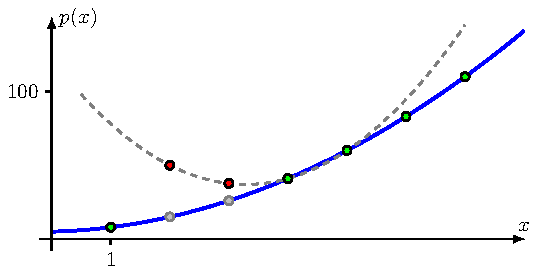
\includegraphics[width=0.5\textwidth]{papers/reedsolomon/images/polynom2}
    %% polynome
%-------------------

\documentclass[tikz]{standalone}
\usepackage{amsmath}
\usepackage{times}
\usepackage{pgfplots}


\begin{document}
% Teiler für das Skalieren der Grafik /40
\newcommand{\teiler}{40}


%//////////////////////////////////////

\begin{tikzpicture}[>=latex,thick]
	\draw[color=blue, line width=1.4pt] 
	plot[domain=0:8, samples=100]
	({\x},{(2*\x^2+1*\x+5)/\teiler});

	\draw[->] (-0.2,0) -- (8,0) coordinate[label={$x$}];
	\draw[->] (0,-0.2) -- (0,150/\teiler) coordinate[label={right:$p(x)$}];
	
	\def\punkt#1{
		\fill[color=green] #1 circle[radius=0.08];
		\draw #1 circle[radius=0.07];
	}

	\def\hellpunkt#1{
		\fill[color=lightgray] #1 circle[radius=0.08];
		\draw[gray] #1 circle[ radius=0.07];
	}
	
	\draw[color=gray,line width=1pt,dashed] 
	plot[domain=0.5:7, samples=100]
	({\x},{(7.832*\x^2-51.5*\x+121.668)/\teiler});


	\punkt{(1,8/\teiler)}
	\hellpunkt{(2,15/\teiler)}
	\hellpunkt{(3,26/\teiler)}
	\punkt{(4,41/\teiler)}
	\punkt{(5,60/\teiler)}
	\punkt{(6,83/\teiler)}
	\punkt{(7,110/\teiler)}
	

	
	\def\erpunkt#1{
		\fill[color=red] #1 circle[radius=0.08];
		\draw #1 circle[radius=0.07];
	}
	\erpunkt{(2,50/\teiler)}
	\erpunkt{(3,37.66/\teiler)}

	\draw(0,100/\teiler) -- (-0.1,100/\teiler) coordinate[label={left:$100$}];
	\draw(1,0) -- (1,-0.1) coordinate[label={below:$1$}];		
\end{tikzpicture}
\end{document}

	\caption{Polynom \eqref{reedsolomon:equation1}}
	\label{fig:polynom}
\end{figure}

\subsection{Beispiel}
Für das Beispeil aus der Gleichung \eqref{reedsolomon:equation1},
ist ein Polynome zweiten Grades durch drei Punkte eindeutig bestimmbar.
Hat es Fehler in der Übertragunge gegeben, kann man diese erkennen,
da alle Punkte, die korrekt sind, auf dem Polynom liegen müssen.
Ab wie vielen Fehler ist das Polynom nicht mehr erkennbar beim Übertragen von 7 Punkten?
Bei 2 Fehlern kann man noch eindeutig bestimmen, dass das Polynom mit 4 Punkten,
gegenüber dem mit 5 Punkten falsch liegt.\ref{fig:polynom}
Werden es mehr Fehler kann nur erkennt werden, dass das Polynom nicht stimmt.
Das orginale Polynom kann aber nicht mehr gefunden werden.
Dafür sind mehr übertragene Werte nötig.

\section{Fehlerbestimmung
\label{reedsolomon:section:Fehlerbestimmmung}}
So wird ein Muster indentifiziert, welches genau vorherbestimmen kann,
wie gross das Polynom sein muss und wie viele Übertragungspunkte gegeben werden müssen.
Um zu bestimmen wie viel Fehler erkennt und korriegiert werden können.
Die Anzahl Zahlen (Daten, ab hier verwenden wir das Wort Nutzlast),
die Entschlüsselt werden sollen, brauchen die gleiche Anzahl an  Polynomgraden, beginnend bei Grad 0. ( \( k-1 \) )
Für die Anzahl an Übertragungspunkte, muss bestimmt werden wieviel Fehler erkennt und korrigiert werden sollen.
Mit Hilfe der Tabelle, sieht man das es bei $t$ Fehlern und $k$ Nutzlast Zahlen,
$k+2t$ Punkte übertragen werden müssen.

\begin{center}
    \begin{tabular}{ c c c } 
        \hline
        Nutzlas & Fehler & Übertragen \\
        \hline 
        3 & 2 & 7 Werte eines Polynoms vom Grad 2 \\ 
        4 & 2 & 8 Werte eines Polynoms vom Grad 3 \\
        3 & 3 & 9 Werte eines Polynoms vom Grad 2 \\ 
        \hline
        $k$ & $t$ & $k+2t$ Werte eines Polynoms vom Grad $k-1$ \\ 
        \hline
    \end{tabular}
\end{center}

Ein toller Nebeneffekt ist das dadurch auch $2t$ Fehler erkannt werden. 
Um zurück auf unser Beispiel zu kommen, 
können von den 7 Übertragungspunkten bis zu $2t = 2\cdot2 = 4 $ Punkten falsch liegen 
und es wird kein eindeutiges Polynom zweiten Grades erkannt, und somit die Nutzlast Daten als fehlerhaft deklariert.
Um aus den Übertragenen Zahlen wieder die Nutzlastzahlen zu bekommen könnte man eine Polynominterpolation anwenden,
doch die Punkte mit Polynominterpolation zu einem Polynom zu rekonstruieren ist schwierig und Fehleranfällig.

